\chapter{Results: solar flares}

\textbf{colocar resultados finales de las iteraciones de LS con residual y plots de comparacion de ambos metodos}

In this chapter different data sets will be studied using the two presented methods for the \textit{BGSEES} algorithm: the \textbf{Least Squares} and \textbf{Decrease Range} methods. 

The aim of the chapter is to test them against each other and using different parameters to see which method yields the best result

The algorithm is tested using data from Solar flares, for these, the ti files of days when a flare had taken place were used to compare the results. The data was filtered around the time of the flare (30 minutes before and after, if there was an exact moment in time).
 
Below is the list of times (\textit{year.day.seconds}) of the different flares we studied. The seconds are either an exact moment in time or a range used in the plots of the papers the flares are listed in.

Flares listed in \textit{"GNSS measurement of EUV photons flux rate during strong and mid solar flares"}\cite{hernandez2012gnss}

\begin{itemize}
	\item 2003.301.39777
	\item 2003.308.71000-71100
	\item 2005.020.24200-24400
%	\item 2006.340.67300-67500
	\item 2011.210.44134
%	\item 2011.216.13908
\end{itemize}

And those listed in \textit{"GPS as a solar observational instrument: Real-time estimation of EUV photons flux rate during strong, medium, and weak solar flares"}\cite{singh2015gps}

\begin{itemize}
%	\item 2001.334.3700-4000
	\item 2001.347.51800-52200
	\item 2002.196.72240
%	\item 2004.204.27800-28000
%	\item 2004.310.41370
%	\item 2004.313.52500
	\item 2005.258.30990
	\item 2012.066.4400-4700
	\item 2012.130.50600-51000
	\item 2012.297.11600-12000
%	\item 2013.310.35970
\end{itemize}

To perform this study, the best epoch within the given range is found using the mean VTEC, as shown in chapter 5. The data is then filtered using this epoch and the algorithm is executed using the necessary parameters, the studied factors are:

The \textbf{execution time} of the algorithm and the \textbf{absolute error} of the estimation, obtained by computing the angle between correct Sun position\footnote{The correct Sun position at that moment is obtained from the data, it is one of the many fields the ti files contain} and the estimated location, using the same operations we've used in previous chapters to compute the angle. 

The ti files that contain data for the entire day are filtered using this bash script, which has a list with the information of each file to be filtered: the name of the original file and the upper and lower limits of time (or a specific moment used to compute the limits). It then filters each file using a simple AWK one-line script that checks the field with the time:

\begin{minipage}{\linewidth}
	\begin{lstlisting}[language=Bash, caption=Filtering the ti file]
#!/bin/bash	
	
strings=(
	'2003.301,36000,41400'
	'2011.210,44134'
	[..All the filenames..] 
	'2012.297,11600,12000'
)
tiDataFolder="/home/mbdavid2/Documents/dataTi/"

for i in "${strings[@]}"; do
	dataInfo="$i"
	
	# Split the information
	arrayInfo=(${dataInfo//,/ })
	
	# Use the range if specified, compute it otherwise
	if [ ${#arrayInfo[@]} = 2 ]; then
		let lowerLimit="${arrayInfo[1]}"-1800
		let upperLimit="${arrayInfo[1]}"+1800
	else
		let lowerLimit="${arrayInfo[1]}"
		let upperLimit="${arrayInfo[2]}"
	fi
	
	# Name the file according to the parameters
	tiDataFile="ti.""${arrayInfo[0]}"
	outputFileName="$tiDataFile"".""$lowerLimit""-""$upperLimit"
	
	# Filter and compress
	zcat "$tiDataFolder""originals/""$tiDataFile" 
	| gawk -v lower="$lowerLimit" -v upper="$upperLimit" 
	'{/a/; if ($3 >= lower/3600 && $3 <= upper/3600) {print $0;}}' 
	> "$tiDataFolder""$outputFileName"
	gzip -f "$tiDataFolder""$outputFileName" # -f to force overwrite
done\end{lstlisting}
\end{minipage}

The study is divided in three categories, based on the method used to discard outliers from the input data:

\begin{itemize}
	\item Using the data from \textbf{all IPPs} without filtering out any outliers
	\item Using a \textbf{cutoff value} for \textbf{all the VTEC data} that will be used for the computations of the algorithm
	\item Using \textbf{linear fit} for the Decreasing Range method to discard outliers and \textbf{multiple iterations} for the Least Squares method to try to improve the solution, both presented in their respective chapters.
\end{itemize}

\clearpage

\section{Using all available data}

For this first test, all the data from the ti file is used: in the case of the Decreasing Range (DR) method, all the VTEC values that could be invalid are used to compute the correlation, and in the case of the Least Squares (LS) method, all are used for the equations of the system.

\begin{table}[h!]
	\centering
	\def\arraystretch{1.2}
	\begin{tabular}{|c c c|} 
		\hline
		Data set & Error (º) & Time (s) \\ [0.3ex] 
		\hline\hline
		2001.347 & 113.813 & 1.03879 \\
		\hline
		2002.196 & 83.5147 & 0.26934 \\
		\hline
		2003.301 & 24.6405 & 1.07813 \\
		\hline
		2003.308 & 128.59 & 0.971644 \\
		\hline
		2005.020 & 20.1031 & 0.916863 \\
		\hline
		2005.258 & 91.3298 & 0.498707 \\
		\hline
		2011.210 & 90.5716 & 1.46812 \\
		\hline
		2012.066 & 133.236 & 2.30571 \\
		\hline
		2012.130 & 162.888 & 2.49292 \\
		\hline
		2012.297 & 78.487 & 0.789705 \\
		\hline
		Total & 927.174 & 11.8299 \\
		\hline
	\end{tabular}
	\quad\quad\quad
	\begin{tabular}{|c c c|} 
		\hline
		Data set & Error (º) & Time (s) \\ [0.3ex] 
		\hline\hline
		2001.347 & 106.064 & 0.0175844 \\
		\hline
		2002.196 & 66.2043 & 0.0158694 \\
		\hline
		2003.301 & 42.2689 & 0.0154119 \\
		\hline
		2003.308 & 55.4949 & 0.326298 \\
		\hline
		2005.020 & 124.218 & 0.14858 \\
		\hline
		2005.258 & 111.073 & 0.0264138 \\
		\hline
		2011.210 & 98.776 & 0.0558694 \\
		\hline
		2012.066 & 64.186 & 0.0143492 \\
		\hline
		2012.130 & 73.1871 & 0.0321778 \\
		\hline
		2012.297 & 47.0189 & 0.00680915 \\
		\hline\hline
		Total & 788.491 & 0.659363 \\
		\hline
	\end{tabular}
	\caption{Estimation error and execution time for different data sets using the DR (left) and LS (right) methods without any filter}
\end{table}

\subsection{Discussion}

The main problem of this method is that outliers can cause the computation of the mean to be unstable, which causes the algorithm to use incorrect epochs.

Furthermore, the outliers can cause numerical instability in some of the methods' computations, if one has a large value, for example, the computation of the correlation relies on the sum of the square of the VTEC value, so the total can lead to incorrect results because of the rapid increase of this variable.

Additionally, the LS method is significantly faster: all data sets together add up to a total execution time of less than one second, whilst the DR method needs that time or even more for almost each of the data sets.

TODO: Comentar el tema de que no esperabamos que fuera perfecto, pero de hecho el siguiente section mejora: (se comenta algo parecido en la conclusion del capitulo)
Considering that this is a new method to detect flares, however, this could have been the case in general (the detection could not have been possible, or at least not with enough precision

\section{Direct VTEC filter}

Although this is a very simple approach to discard outliers, we decided to test it because the value of the Delta VTEC does not usually surpass values such as 0.8, only some IPPs might present values like this, due to other interferences in the satellite data. The flare from the day 301 of 2003, for example, studied in previous chapters, is one of the most powerful flares ever recorded, and the peak value of the Delta VTEC is 0.4.

These are the results of the execution using a cutoff value of 0.7. This value was selected as it is the one that yielded the best results in a range of 0.3 to 1:

\begin{table}[h!]
	\centering
	\def\arraystretch{1.2}
	\begin{tabular}{|c c c|} 
		\hline
		Data set & Error (º) & Time (s) \\ [0.3ex] 
		\hline\hline
		2001.347 & 3.53947 & 1.03243 \\
		\hline
		2002.196 & 27.6877 & 0.287287 \\
		\hline
		2003.301 & 3.93239 & 1.36538 \\
		\hline
		2003.308 & 131.366 & 0.891328 \\
		\hline
		2005.020 & 64.8737 & 0.551884 \\
		\hline
		2005.258 & 48.7806 & 1.00214 \\
		\hline
		2011.210 & 126.204 & 1.23266 \\
		\hline
		2012.066 & 75.1081 & 1.85402 \\
		\hline
		2012.130 & 56.7937 & 2.42187 \\
		\hline
		2012.297 & 1.46042 & 2.86145 \\
		\hline
		Total & 539.746 & 13.5005 \\
		\hline
	\end{tabular}
	\quad\quad\quad
	\begin{tabular}{|c c c|} 
		\hline
		Data set & Error (º) & Time (s) \\ [0.3ex] 
		\hline\hline
		2001.347 & 3.41832 & 0.0114944 \\
		\hline
		2002.196 & 46.578 & 0.00492704 \\
		\hline
		2003.301 & 4.57509 & 0.00724225 \\
		\hline
		2003.308 & 141.865 & 0.378145 \\
		\hline
		2005.020 & 38.3263 & 0.129509 \\
		\hline
		2005.258 & 1.88011 & 0.0103007 \\
		\hline
		2011.210 & 38.5213 & 0.0603164 \\
		\hline
		2012.066 & 70.1063 & 0.0251154 \\
		\hline
		2012.130 & 9.26238 & 0.0518934 \\
		\hline
		2012.297 & 3.00704 & 0.0392889 \\
		\hline
		Total & 357.54 & 0.718233 \\
		\hline
	\end{tabular}
	\caption{Estimation error and execution time for different data sets using the DR (left) and LS (right) methods with a cutoff filter}
\end{table}

\subsection{Discussion}

As we can see, there has been a significant improvement in for both methods by discarding outliers, and because this filter is applied when performing the filtering by time of the data, it doesn't have an impact on the complexity of the execution. 

Because the direct filter yields significantly better results for both cases, the next sections use it for filtering the first traversal of the data, before performing an additional filter to attempt to discard outliers.

\clearpage

\section{Decreasing range: linear fit}

This approach, introduced in chapter 6, discards outliers by finding the line that fits the data set and discarding outliers based on a sigma parameter. This filter can be performed several times (the number of iterations). The results of the decreasing range method using a sigma of 3 and 4 iterations (the best combination of those values in a range from 1 to 10) is shown below

\begin{table}[h!]
	\centering
	\def\arraystretch{1.2}
	\begin{tabular}{|c c c|} 
		\hline
		Data set & Error (º) & Time (s) \\ [0.5ex] 
		\hline\hline
		2001.347.gz & 3.66657 & 45.4151 \\
		\hline
		2002.196.gz & 30.9237 & 42.6182 \\
		\hline
		2003.301.gz & 3.57674 & 51.7222 \\
		\hline
		2003.308.gz & 79.3679 & 43.6955 \\
		\hline
		2005.020.gz & 68.911 & 37.3023 \\
		\hline
		2005.258.gz & 22.6375 & 50.5795 \\
		\hline
		2011.210.gz & 19.7344 & 55.8291 \\
		\hline
		2012.066.gz & 84.3076 & 31.9302 \\
		\hline
		2012.130.gz & 21.896 & 42.326 \\
		\hline
		2012.297.gz & 0.679492 & 53.7369 \\
		\hline
		Total & 335.701 & 455.155 \\
		\hline
	\end{tabular}
	\caption{Results for different data sets using linear fit with the DR method}
\end{table}

\subsection{Discussion}

While this approach improves upon the solution of the Least Squares method, it requires significantly higher execution time (each execution takes almost a minute).

\clearpage

\section{Least Squares: Iterations}

Although we have seen in the previous chapter that the iterations didn't work for a specific case, we decided to test it using all data sets. These are the results of executing the algorithm with 10 iterations, saving the result of the best iteration:

\begin{table}[h!]
	\centering
	\def\arraystretch{1.2}
	\begin{tabular}{|c c c|} 
		\hline
		Data set & Error (º) & Time (s) \\ [0.5ex] 
		\hline\hline
		2001.347.gz & 3.41832 & 0.0194832 \\
		\hline
		2002.196.gz & 46.578 & 0.00818968 \\
		\hline
		2003.301.gz & 4.57509 & 0.0171783 \\
		\hline
		2003.308.gz & 141.865 & 0.366494 \\
		\hline
		2005.020.gz & 38.3263 & 0.141508 \\
		\hline
		2005.258.gz & 1.88011 & 0.0177967 \\
		\hline
		2011.210.gz & 38.5213 & 0.0704044 \\
		\hline
		2012.066.gz & 70.1063 & 0.049831 \\
		\hline
		2012.130.gz & 9.26238 & 0.0711422 \\
		\hline
		2012.297.gz & 3.00704 & 0.0592826 \\
		\hline
		Total & 357.54 & 0.82131 \\
		\hline
	\end{tabular}
	\caption{Results for different data sets}
	\label{tab:lsDirect}
\end{table}

\subsection{Discussion}

As we can see, the results in terms of estimation error are exactly the same as the ones seen in table \ref{tab:lsDirect} with a slight increase in execution time due to the number of iterations. Because there is no improvement with consecutive iterations, the algorithm just keeps the best result from the first one, hence the same results.

\subsection{Error comparison}

Despite the fact that using this approach does not improve the results, it can be interesting to see how the covariance matrix error evolves compared to the real error for all the studied data sets, figure \ref{fig:comparisonErrors} shows a comparison for all the tested data sets the real error and LS error:

\begin{figure}[!htb]
	\begin{centering}
		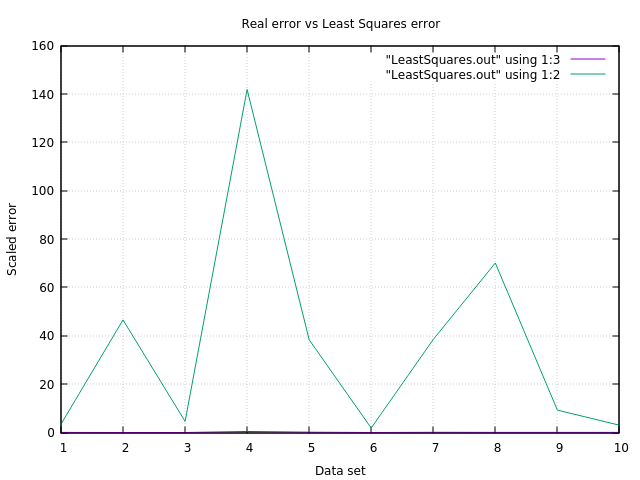
\includegraphics[width=0.5\linewidth]{images/results/comparisonErrors.png}
		\caption{Comparison of the real error (purple) and the estimated Least Squares error (green)}
		\label{fig:comparisonErrors}
	\end{centering}
\end{figure}

As we can see, both functions seem to have similar spikes. If the solution has a large error, it is because the Least Squares method could not provide a good solution with the available data. As we have seen, some of the studied flares are hard to detect for both methods, due to their intensity.

\section{Conclusion}

In this chapter we have seen that working with the entire data set of IPPs does not yield good results, there is too much noise and the results differ considerably from the real position of the Sun. Considering that this is a new method to detect flares, however, this could have been the case in general (the detection could not have been possible, or at least not with enough precision), but using a direct filter for the VTEC values we have seen that some of the data sets yield results with errors as little as 4 degrees.

It can be interesting to see, however, how some data sets still have a high error, due to the nature of the flare (perhaps it was not sufficiently strong to have an impact on the ionosphere), the following plot compares the Least Squares method error of the direct filter approach and using all the data.

We can see

In conclusion, the Decreasing Range method (using linear fit to discard outliers) and the Least Squares method (using a direct filter) provide good results for some of the data sets with powerful flares, therefore, these two methods will

conclusion de todo el chapter? comparar aqui ambos metodos, \textbf{hacer plot de comparacion del error y el tiempo para ver que ambos tienen errores en los mismos flares debido a la debilidad de algunos}

Decidir cual es el mejor metodo para usar en stellar flares? pero decir que igualmente probamos con ambos

